\begin{figure}[t]
\centering
\subfigure[Line Graph]{
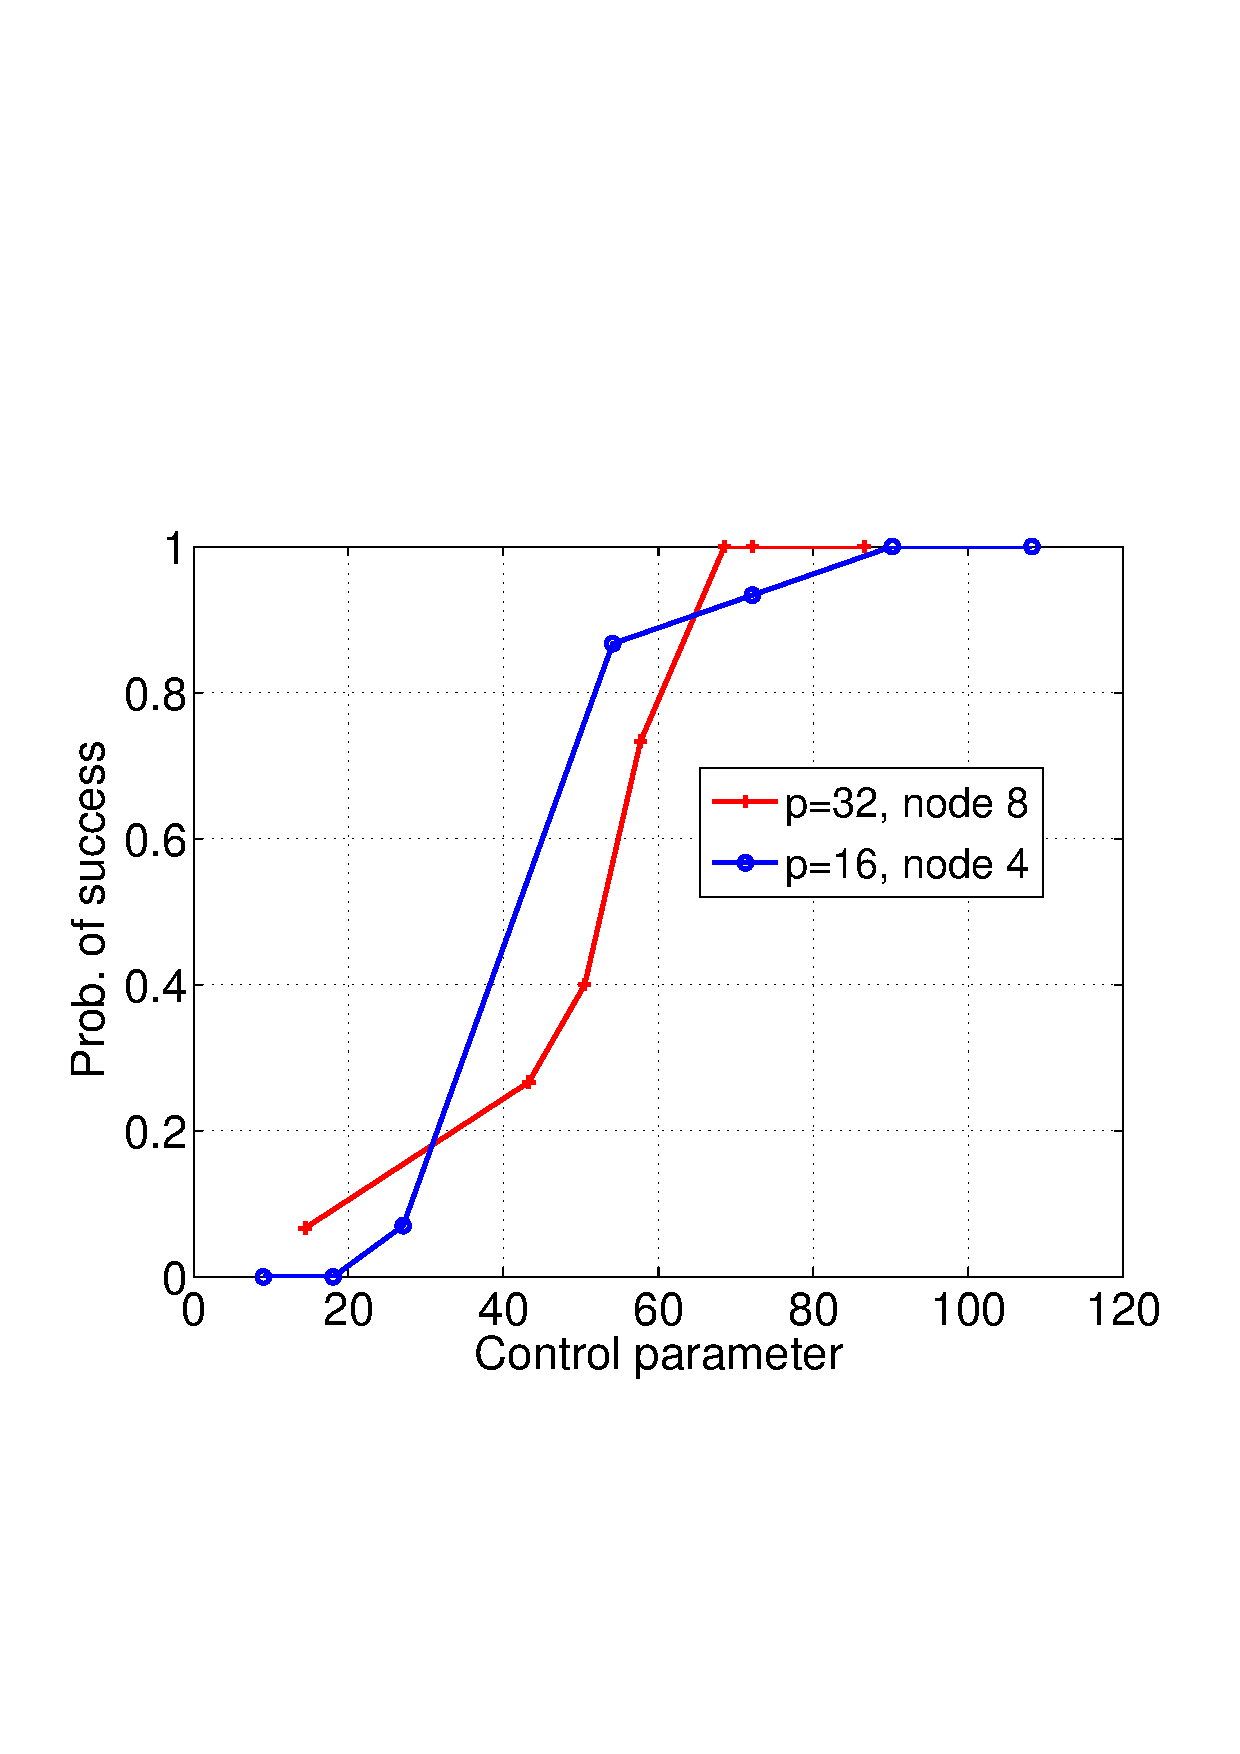
\includegraphics[scale=0.3]{figures/nbdRecovery-chain}
% \label{fig:graphtype:line}
}
\subfigure[Grid]{
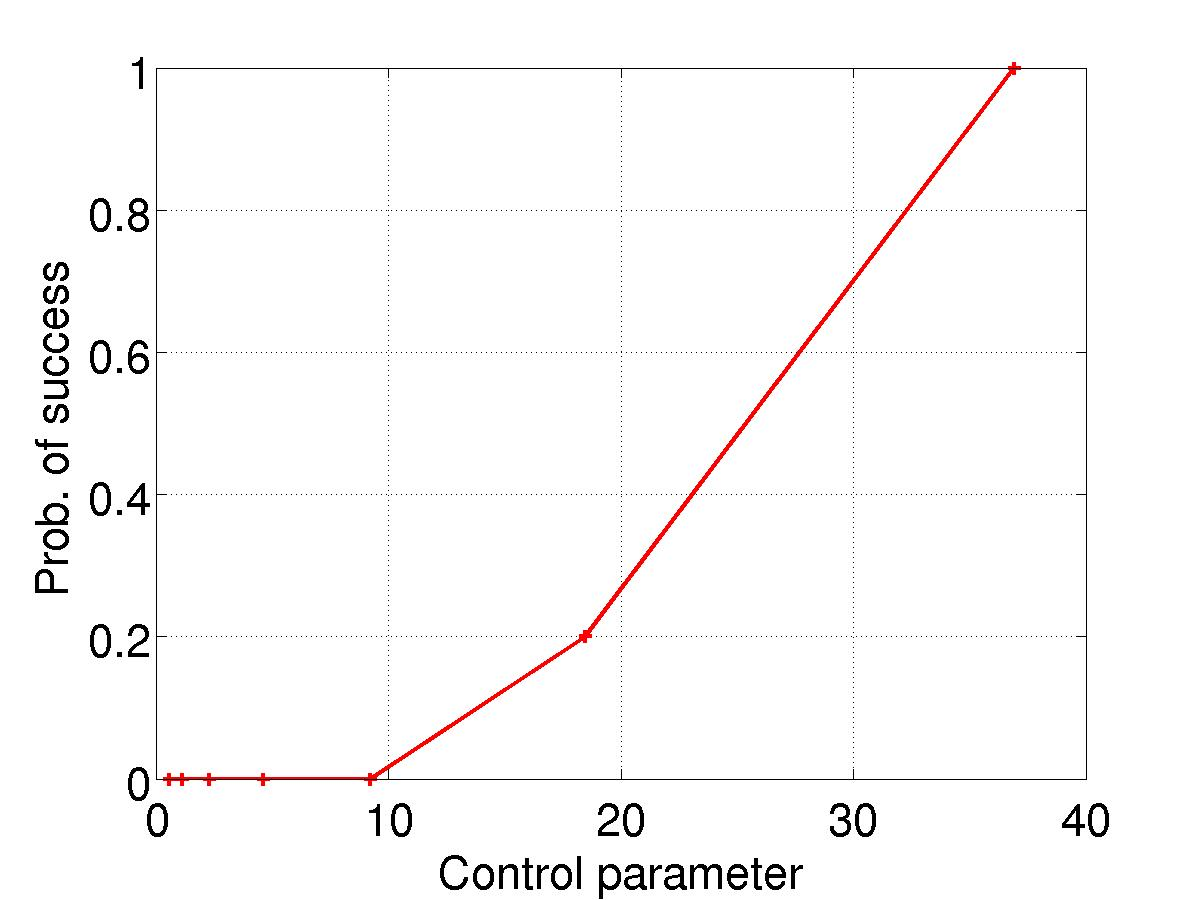
\includegraphics[scale=0.3]{figures/grid16nNode6}
% \label{fig:graphtype:grid}
}
\label{fig:neighborhoodrecovery}
\caption{Probability of success \small$\mathbb{P}[\widehat{\N}(\svert) = \N(\svert)]$\normalsize versus the control parameter $\beta(n, p, d) = \frac{n}{10 d \log(p)}$ for discrete graphical models on a Line Graph and a Grid.}
 
\end{figure}

\begin{figure}[t]
\centering
\subfigure[Line Graph]{
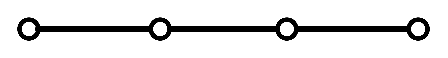
\includegraphics[scale=0.3]{Drawing1.eps}
\label{fig:graphtype:line}
}
\subfigure[Grid]{
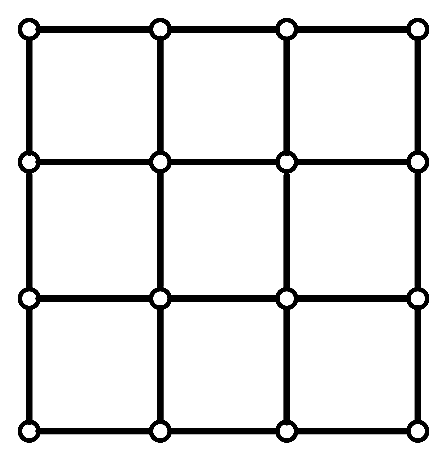
\includegraphics[scale=0.3]{Drawing2.eps}
\label{fig:graphtype:grid}
}
\subfigure[Three-Way]{
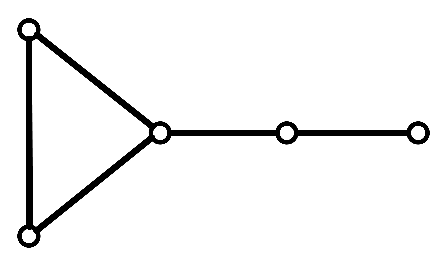
\includegraphics[scale=0.3]{Drawing3.eps}
\label{fig:graphtype:threeway}
}
\label{fig:graphtype}
\caption[Graph Types:]{Line graph \subref{fig:graphtype:line} and Grid \subref{fig:graphtype:grid} are used in studying pairwise graphical model selection. Three-way graph \subref{fig:graphtype:threeway} is used for studying higher-order graphical model selection.}
\end{figure}


\begin{figure}[t]
\centering
\includegraphics[scale=0.3]{figures/spade16nNode3.eps}
\label{fig:higherOrder}
\caption{Probability of success \small$\mathbb{P}[\widehat{\N}(\svert) = \N(\svert))]$\normalsize versus the control parameter $\beta(n, p, d) = \frac{n}{10 d \log(p)}$ for a higher order discrete graphical model on a Three-way graph.}
\end{figure}

\section{Experiments}
\noindent In this section, we report a set of synthetic experiments investigating the consequences of the main theorems. These results illustrate the behavior of the structure learning algorithm on various types of graphs. We fix the size of the alphabet $m=3$. For a given graph type, we pick a pairwise parameter set $\Theta^*$. We generate $n$ samples according to the probability distribution corresponding to $\Theta^*$. Then, we solve \eqref{EqnPairwiseGroup} and compare the graph corresponding to the solution with the original graph. If the two graphs are identical, we declare that the algorithm has succeeded.


{\bf Pairwise Model:} We consider two different classes of graphs: line graphs and grids (Fig.~\ref{fig:graphtype}). In particular, we consider line graphs of size $p=16,32$ and a grid of size $\sqrt{p}\times \sqrt{p} = 16$. In each of these cases, the parameter vector $\Theta^*$ is generated by setting each non-zero entry $\theta^*_{\svert t;jk} \in [-0.5, 0.5]$ for the line graphs and $\theta^*_{\svert t;jk} \in [0, 5]$ for the grid unfirmly at random. To estimate the probability of success, we use $15$ batches of samples drawn from the distribution specified by $\Theta^*$. We consider two types of simulations:

%\begin{itemize}

%\item 
\noindent {\bf Neighborhood Recovery:} Here, we focus on the recovery of the neighborhood of a particular node in a graph. Fixing a sample batch, for each pair $(p,n)$, we set $\regpar_n=K\left(\sqrt{\frac{p-1}{n}}+\frac{m-1}{4\sqrt{n}}\right)$, where $K$ is the constant chosen by cross validation. We compare the graph induced by $\widehat{\Theta}_{K^*}$ with the graph induced by $\Theta^*$ to get the probability of success. Fig~\ref{fig:neighborhoodrecovery} shows the probability of success in neighborhood recovery. Notice that for different values of $n$ and $p$, the phase transition graphs stack on the top of each other; this shows that the scaling of the samples $n$ is correct.

%\item {\bf Graph Recovery:} We then, investigate the recovery of the whole graph. Solving the optimization problem \eqref{EqnPairwiseGroup} for all nodes, we declare success if the recovered neighborhood of all nodes exactly matches the true neighborhood. Fig.~\ref{fig:graphrecovery} shows the probability of success in recovery of the graph structure using our method. 
%\end{itemize}


{\bf Higher-Order Model:} In this case, we consider a graph with higher order dependencies and try to estimate it using the pairwise model. We consider the three-way graph (triangle + line graph of size $p-2$) shown in Fig~\ref{fig:graphtype:threeway}. There is only one three-way factor involving three nodes. The rest of the graph is characterized by pairwise parameters. Solving \eqref{EqnGroupHigherOrder}, we investigate the probability of success for neighborhood recovery of the node that connects the line graph and the triangle. Fig.~\ref{fig:higherOrder} illustrates the result.

